\documentclass[12pt]{article}
\setcounter{secnumdepth}{3}

\usepackage[margin=0.5in]{geometry} 
\usepackage{amsmath,amsthm,amssymb,color}
\usepackage{graphicx}
\usepackage{mathtools}
\usepackage[section]{placeins}
\usepackage{listings}
\usepackage{mathdots}
\usepackage{centernot}
\usepackage{algorithm}
\usepackage[noend]{algpseudocode}
\usepackage{csquotes}
\usepackage[table,xcdraw]{xcolor}
\usepackage{booktabs}
\usepackage{cite}
\usepackage{enumerate}
\usepackage{tikz}
\usetikzlibrary{calc}
\usepackage{bbm}
\usetikzlibrary{arrows, shapes}
\usetikzlibrary{patterns}
\usepackage{natbib}
\usepackage{relsize}
\usepackage{booktabs}
\usetikzlibrary{decorations.pathreplacing}
\allowdisplaybreaks


\usepackage{hyperref}
\hypersetup{
    colorlinks,
    citecolor=black,
    filecolor=black,
    linkcolor=black,
    urlcolor=black
}

\DeclarePairedDelimiter\ceil{\lceil}{\rceil}
\DeclarePairedDelimiter\floor{\lfloor}{\rfloor}
 
\newcommand\scalemath[2]{\scalebox{#1}{\mbox{\ensuremath{\displaystyle #2}}}}

\newcommand{\N}{\mathcal{N}}
\newcommand{\Z}{\mathbb{Z}}
\newcommand\independent{\protect\mathpalette{\protect\independenT}{\perp}}
\def\independenT#1#2{\mathrel{\rlap{$#1#2$}\mkern2mu{#1#2}}}

\theoremstyle{plain}
\newtheorem{thm}{Theorem}%[section]
\theoremstyle{plain}
\newtheorem{lem}{Lemma}%[section]
\theoremstyle{plain}
\newtheorem{prop}{Proposition}%[section]
\theoremstyle{plain}
\newtheorem{cor}{Corollary}%[thm]
\theoremstyle{plain}
\newtheorem{defin}{Definition}%[section]
\theoremstyle{remark}
\newtheorem{rem}{Remark}%[section]
\theoremstyle{plain}
\newtheorem{exe}{Exercise}%[section]
\theoremstyle{plain}
\newtheorem{exa}{Example}%[section]
\theoremstyle{plain}
\newtheorem{fact}{Fact}%[section]
\theoremstyle{discussion}
\newtheorem{discussion}{Discussion}%[section]
\theoremstyle{plain}
\newtheorem{conj}{Conjecture}%[section]

\newcommand{\wtil}{\widetilde}
\newcommand{\inte}{\mathrm{int}}
\newcommand{\iid}{\stackrel{\text{iid}}{\sim}}
\newcommand{\eqe}{\stackrel{\cdot}{=}}
\newcommand{\ft}{\mathcal{F}}
\newcommand{\mm}{S}
\newcommand{\spa}{\mathrm{Spa}}
\newcommand{\sm}{\widehat{\mathrm{M}}}
\newcommand{\dou}{\mathrm{Doub}}
\newcommand{\cir}{\mathrm{Circ}}
\newcommand{\supp}{\mathrm{supp}}
\newcommand{\M}{\mathcal{M}}
\newcommand{\F}{\mathbb{F}}
\newcommand{\mR}{\mathbb{R}}
\newcommand{\mN}{\mathbb{N}}
\newcommand{\mZ}{\mathbb{Z}}
\newcommand{\mC}{\mathbb{C}}
\newcommand{\mQ}{\mathbb{Q}}
\newcommand{\mF}{\mathbb{F}}
\newcommand{\iim}{\mathrm{Im}\:}
\newcommand{\re}{\mathrm{Re}\:}
\newcommand{\tr}{\mathrm{tr}}
\newcommand{\Corr}{\mathrm{corr}}
\newcommand{\Cov}{\mathrm{cov}}
\newcommand{\pp}{\mathbb{P}}
\newcommand{\E}{\mathbb{E}}
\DeclareMathOperator{\Var}{Var}
\newcommand{\e}{\varepsilon}
\newcommand{\ent}{h}
\newcommand{\info}{I}
\newcommand{\rank}{\mathrm{rank}}
\newcommand{\nullity}{\mathrm{nullity}}
\DeclareMathOperator{\diag}{diag}
\newcommand{\cS}{\mathcal{S}}
\newcommand{\cT}{\mathcal{T}}
\newcommand{\X}{\mathcal{X}}
\newcommand{\Y}{\mathcal{Y}}
\newcommand{\I}{\mathcal{I}}
\newcommand{\D}{\mathcal{D}}
\newcommand{\C}{\mathcal{C}}
\newcommand{\B}{\mathcal{B}}
\newcommand{\Po}{\mathcal{P}}
\newcommand{\Tr}{\text{Trace}}
\newcommand\mapsfrom{\mathrel{\reflectbox{\ensuremath{\mapsto}}}}


\begin{document}

\begin{figure}
\begin{center}
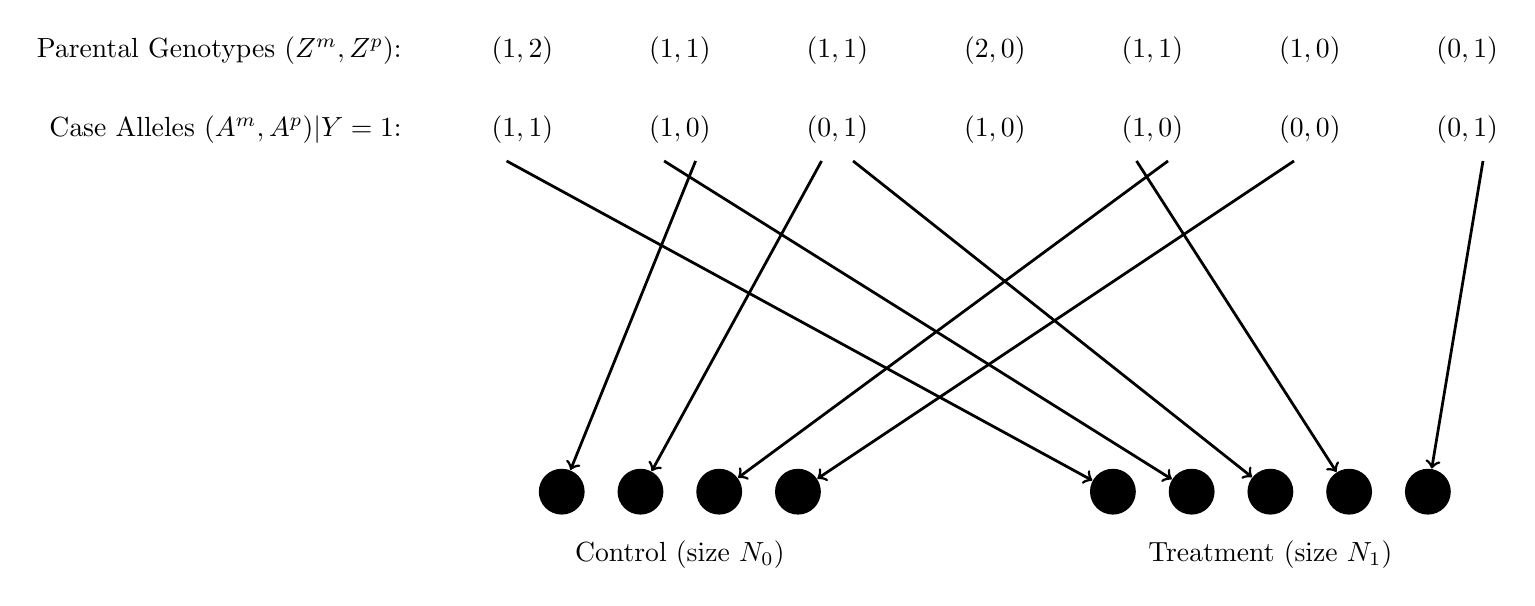
\begin{tikzpicture}[scale = 1]

\tikzstyle{vertex_P}=[rectangle,fill=blue, opacity = 0.5, text width = 6mm, text height = 6mm]
\tikzstyle{vertex_M}=[diamond,fill=red, opacity = 0.5, text width = 7mm]
\tikzstyle{vertex_t}=[circle,fill=black, opacity = 1, text width = 3mm]
\tikzstyle{vertex_c}=[circle,fill=black, opacity = 1, text width = 3mm]

\coordinate (Y1) at (-6, 3);
\coordinate (Y2) at (-4, 3);
\coordinate (Y3) at (-2, 3);
\coordinate (Y4) at (0, 3);
\coordinate (Y5) at (2, 3);
\coordinate (Y6) at (4, 3);
\coordinate (Y7) at (6, 3);
\coordinate (y1m) at (-6.2, 3.6);
\coordinate (y2m) at (-4.2, 3.6);
\coordinate (y3m) at (-2.2, 3.6);
\coordinate (y4m) at (-0.2, 3.6);
\coordinate (y5m) at (1.8, 3.6);
\coordinate (y6m) at (3.8, 3.6);
\coordinate (y7m) at (5.8, 3.6);
\coordinate (y1p) at (-5.8, 3.6);
\coordinate (y2p) at (-3.8, 3.6);
\coordinate (y3p) at (-1.8, 3.6);
\coordinate (y4p) at (0.2, 3.6);
\coordinate (y5p) at (2.2, 3.6);
\coordinate (y6p) at (4.2, 3.6);
\coordinate (y7p) at (6.2, 3.6);
\coordinate (T) at (4, -0.8);
\coordinate (C) at (-5, -0.8);
\coordinate (mp) at (-9.77, 4);
\coordinate (H) at (-9.85, 5);


\path
($(T) + (-2 - .5, 0.2)$) node[vertex_t](t1) {}
($(T) + (-1 - .5, 0.2)$) node[vertex_t](t2) {}
($(T) + (0 - .5, 0.2)$) node[vertex_t](t3) {}
($(T) + (1 - .5, 0.2)$) node[vertex_t](t4) {}
($(T) + (2 - .5, 0.2)$) node[vertex_t](t5) {}
($(C) + (-1 + 0.5, 0.2)$) node[vertex_c](c1) {}
($(C) + (0 + 0.5, 0.2)$) node[vertex_c](c2) {}
($(C) + (1 + 0.5, 0.2)$) node[vertex_c](c3) {}
($(C) + (2 + 0.5, 0.2)$) node[vertex_c](c4) {}
($(T) + (-.5, -.6)$) node(treatment) {Treatment (size $N_1$)}
($(C) + (1, -.6)$) node(control) {Control (size $N_0$)}
($(mp)$) node(mp) {Case Alleles $(A^m,A^p)|Y=1$:}
($(Y1) + (0, 1)$) node(g1) {$(1, 1)$}
($(Y2) + (0, 1)$) node(g2) {$(1, 0)$}
($(Y3) + (0, 1)$) node(g3) {$(0, 1)$}
($(Y4) + (0, 1)$) node(g4) {$(1, 0)$}
($(Y5) + (0, 1)$) node(g5) {$(1, 0)$}
($(Y6) + (0, 1)$) node(g6) {$(0, 0)$}
($(Y7) + (0, 1)$) node(g7) {$(0, 1)$};

\path
($(H)$) node(data) {Parental Genotypes $(Z^m,Z^p)$:}
($(Y1) + (0, 2)$) node(g1) {$(1, 2)$}
($(Y2) + (0, 2)$) node(g2) {$(1, 1)$}
($(Y3) + (0, 2)$) node(g3) {$(1, 1)$}
($(Y4) + (0, 2)$) node(g4) {$(2, 0)$}
($(Y5) + (0, 2)$) node(g5) {$(1, 1)$}
($(Y6) + (0, 2)$) node(g6) {$(1, 0)$}
($(Y7) + (0, 2)$) node(g7) {$(0, 1)$};


%arrows
% \draw[->, line width = 1, color = black] (y1m) to [out=270,in=90] (t1);
% \draw[->, line width = 1, color = black] (y2m) to [out=270,in=90] (t2);
% \draw[->, line width = 1, color = black] (y3p) to [out=270,in=90] (t3);
% \draw[->, line width = 1, color = black] (y5m) to [out=270,in=90] (t4);
% \draw[->, line width = 1, color = black] (y7p) to [out=270,in=90] (t5);
% \draw[->, line width = 1, color = black] (y2p) to [out=270,in=90] (c1);
% \draw[->, line width = 1, color = black] (y3m) to [out=270,in=90] (c2);
% \draw[->, line width = 1, color = black] (y5p) to [out=270,in=90] (c3);
% \draw[->, line width = 1, color = black] (y6m) to [out=270,in=90] (c4);

% straight arrow lines
\draw[->, line width = 1, color = black] (y1m) to (t1);
\draw[->, line width = 1, color = black] (y2m) to (t2);
\draw[->, line width = 1, color = black] (y3p) to (t3);
\draw[->, line width = 1, color = black] (y5m) to (t4);
\draw[->, line width = 1, color = black] (y7p) to (t5);
\draw[->, line width = 1, color = black] (y2p) to (c1);
\draw[->, line width = 1, color = black] (y3m) to (c2);
\draw[->, line width = 1, color = black] (y5p) to (c3);
\draw[->, line width = 1, color = black] (y6m) to (c4);

\end{tikzpicture}
\end{center}
\end{figure}

\end{document}